\section{The PicoRV32: System on Chip}
\label{picorv_desc}
The goal of this project is to make a simple demonstrator SoC, with a CPU, memory blocks, and standardized interconnect bus with a basic set of peripherals. This demonstrator chip will then be used to test whether it is possible to create a radiation-tolerant SoC with a reasonable amount of area and power usage. Computing power is not of concern as its use case is targeted toward control and monitoring. RISC-V is an open-source instruction set architecture (ISA) that perfectly fits this application. Many different open-source SoC foundations have been considered and 3 stood out as candidates. Those are the Rocket Chip from UC Berkeley, the PicoSoC, and the Pulpissimo by ETH Zurich. The Rocket chip is a promising chip-building framework in Chisel. The PicoSoC is simple and written in pure Verilog, making it easier to understand. The Pulpissimo is made by ETH which has been collaborating with CERN before and therefore enables more direct communication with the designers. These three have been compared on their power and area usage during post-synthesis. The result of this can be seen in figure \ref{fig:CpuComparison}. Based on this comparison, the PicoSoC is chosen for the demonstrator chip.

\begin{figure}[H]
    \centering
    \begin{subfigure}[b]{0.49\textwidth}
        \centering
        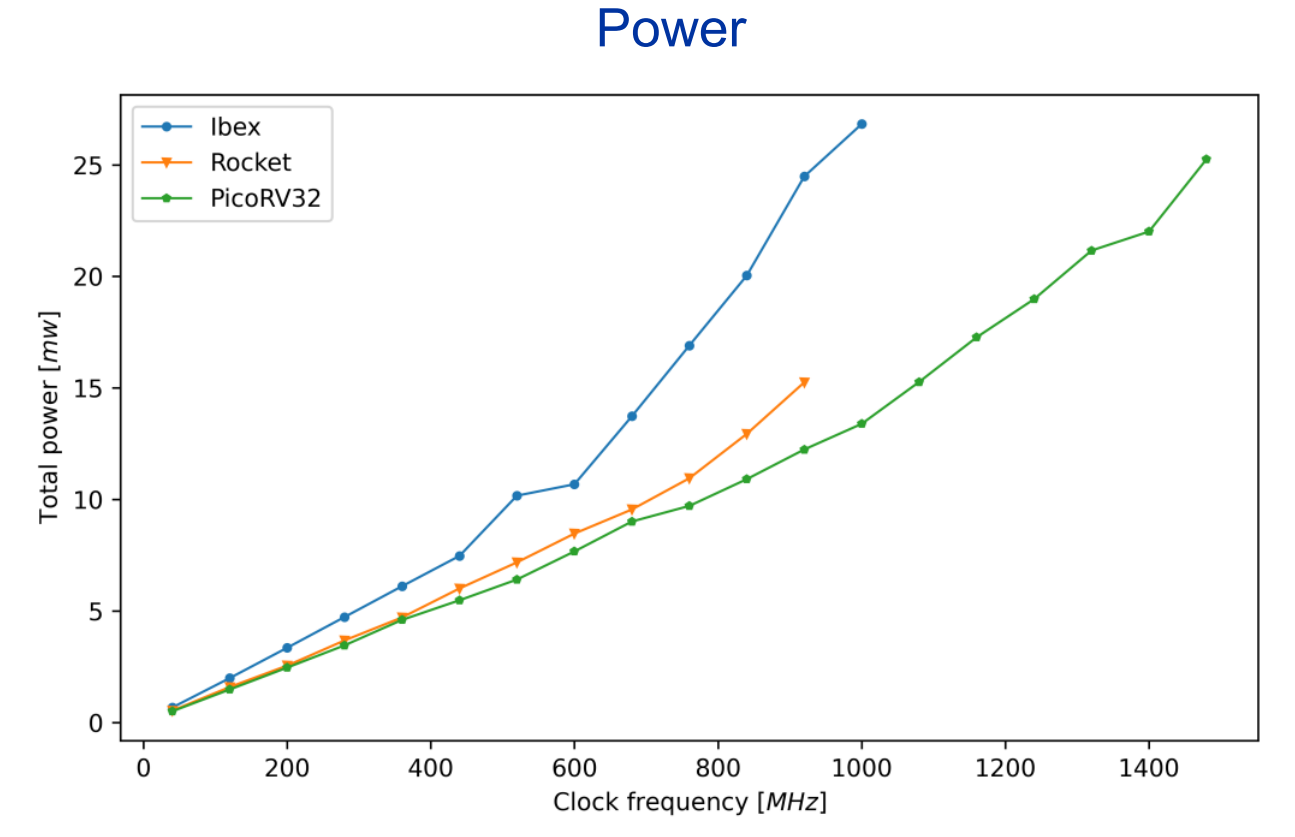
\includegraphics[width=\textwidth]{subfiles/imgs/cpuComparePower.png}
        \caption{}
        \label{fig:cpuComparePower}
    \end{subfigure}
    \hfill
    \begin{subfigure}[b]{0.49\textwidth}
        \centering
        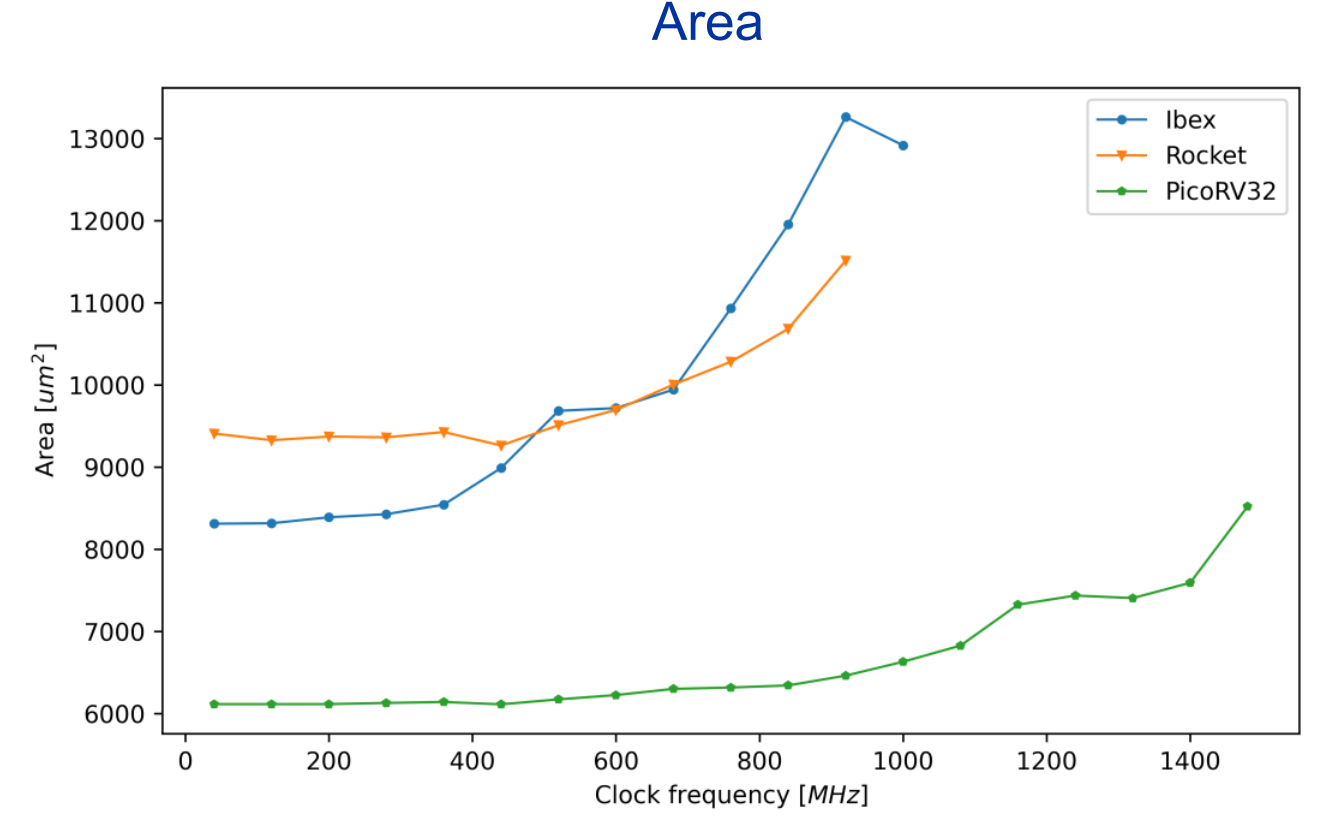
\includegraphics[width=\textwidth]{subfiles/imgs/cpuCompareArea.png}
        \caption{}
        \label{fig:cpuCompareArea}
    \end{subfigure}
    \hfill
    \caption{Shows the post-synthesis power and area comparison of an Ibex, Rocket, and PicoRV32 core.}
    \label{fig:CpuComparison}
\end{figure}

The PicoRV32 SoC is based upon the RISC-V open-source CPU: PicoRV32. This core is meant to be used as a size-optimized auxiliary CPU in an FPGA or ASIC design. It does not have high computational power, but it is small and simple. Due to its simplicity, it is also easier to debug and develop extra features. 

RISC-V is an open-source instruction set architecture (ISA). Its architecture is developed on Reduced Instruction Set Computer (RISC) principles. This is in contrast to the Complex Instruction Set Computer (CISC), to which the commonly known family of x86 ISAs belongs. The two design topologies differ because a CISC instruction often executes several lower-level instructions, while a RISC architecture does not. RISC-V employs a base set of the most needed instruction, while several extensions are available to expand the instruction set. The PicoRV32 is configurable \cite{picorv_nmi_if}. Its instruction base can be based on either RV32I (32-bit, base integer instruction set) or RV32E (32-bit, base integer embedded instruction set). The RV32I is capable of having two extensions added: multiplication (M) and the compressed instruction set (C). There is also an optional built-in interrupts controller. However, this is not based upon the RISC-V standard and is instead custom-built for the PicoRV32. This design choice was made because the RISC-V interrupt handle was extensive and comprehensive, so a simpler IRQ handling with less hardware overhead is available.

At the start of this project, several things were already implemented: The core, two buses, a bridge connecting the two busses, and a temporary memory block. A Native Memory Interface (NMI) connects the core and memory. The NMI is connected to a bridge that is connected to an Advanced Peripheral Bus (APB) interface. Peripherals will be connected to SoC using the APB interface. The state of the SoC at the beginning of this project is visualized in figure \ref{fig:PicoRV32SoC@beginning}.  

\begin{figure}[H]
    \centering
    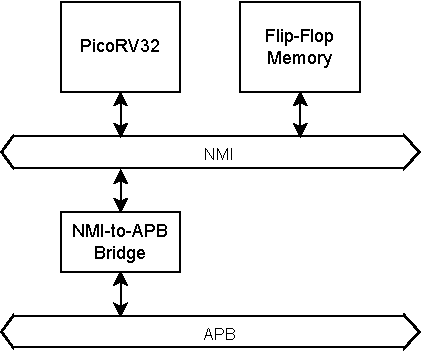
\includegraphics[width=0.5\linewidth]{subfiles/imgs/picorvSOCbeginning.drawio.pdf}
    \caption{Shows the state of the PicoRV32 SoC at the beginning of this project.}
    \label{fig:PicoRV32SoC@beginning}
\end{figure}

A detailed description of the two interfaces used on the buses is now given.

\subsection{Native Memory Interface}
\label{nmi_if}
The NMI is an interface defined by the PicoRV32 \cite{picorv_nmi_if}. It is a simple valid-ready interface bus. It requires five outputs from the PicoRV32 core and two outputs from the slave, which is receiving the transfer. These signals and their functions are described in table \ref{tab:nmi_sig}. This bus is only used to connect the most essential and critical blocks to the core, e.g., memory and bootloader. 


\begin{table}[H]
\centering
\caption{NMI signal descriptions}
\label{tab:nmi_sig}
\begin{tabular}{lll}
\hline
\textbf{Signal} \hspace{1cm} & \textbf{Source} \hspace{1.5cm} & \textbf{Description} \\ \hline
CLK & Clock source & Clock. The transfer is completed on the rising edge. \\ \hline
VALID & PicoRV32 core & \makecell[l]{Valid. The core uses the valid signal to initiate a \\ transfer. All core outputs are stable while valid is high.} \\ \hline
INSTR & PicoRV32 core & \makecell[l]{Instruction fetch. Used by the core to indicate if the \\ memory transfer is an instruction fetch}  \\ \hline
READY & Slave interface & \makecell[l]{Ready. Asserted by the slave when the read data is \\ available and used to acknowledge a write transfer.} \\ \hline
ADDR & PicoRV32 core & \makecell[l]{Address. The core supplies the address which is used by \\ the slave to read or write to the requested cell.} \\ \hline
WDATA & PicoRV32 core & \makecell[l]{Write data. If a write transfer is being performed, the \\ core supplies the data to be written using this bus} \\ \hline
WSTRB & PicoRV32 core & \makecell[l]{Write strobe. If the write strobe is 0, it indicates a read \\ transfer, while it being non-zero indicates a write \\ operation. The write strobe signal is used to write \\ specific bytes of the wdata. It is possible to write 32 bits, \\ the upper 16 bits, the lower 16 bits, or 8 bits.}  \\ \hline
RDATA & Slave interface &  \makecell[l]{Read data. In the case of read transfer, this is the data \\ read from the specified address. When rdata is available, \\ ready is asserted.} \\ \hline
\end{tabular}%

\end{table}

This bus is fully triplicated to achieve radiation hardening. This is decided due to it being critical infrastructure and also the length of this bus being limited since peripheral devices are not connected to this bus. 

\subsection{AMBA APB Interface}
\label{apb_if}
The APB is designed by ARM and is part of the Advanced Microcontroller Bus Architecture (AMBA) protocol family. This protocol has been chosen for the SoC since it is designed for minimal power consumption and reduced interface complexity \cite{apbReference}, which aligns with the goals of the project. The list of signals in the protocol can be seen in figure \ref{fig:apb_signals}.

\begin{figure}[H]
    \centering
    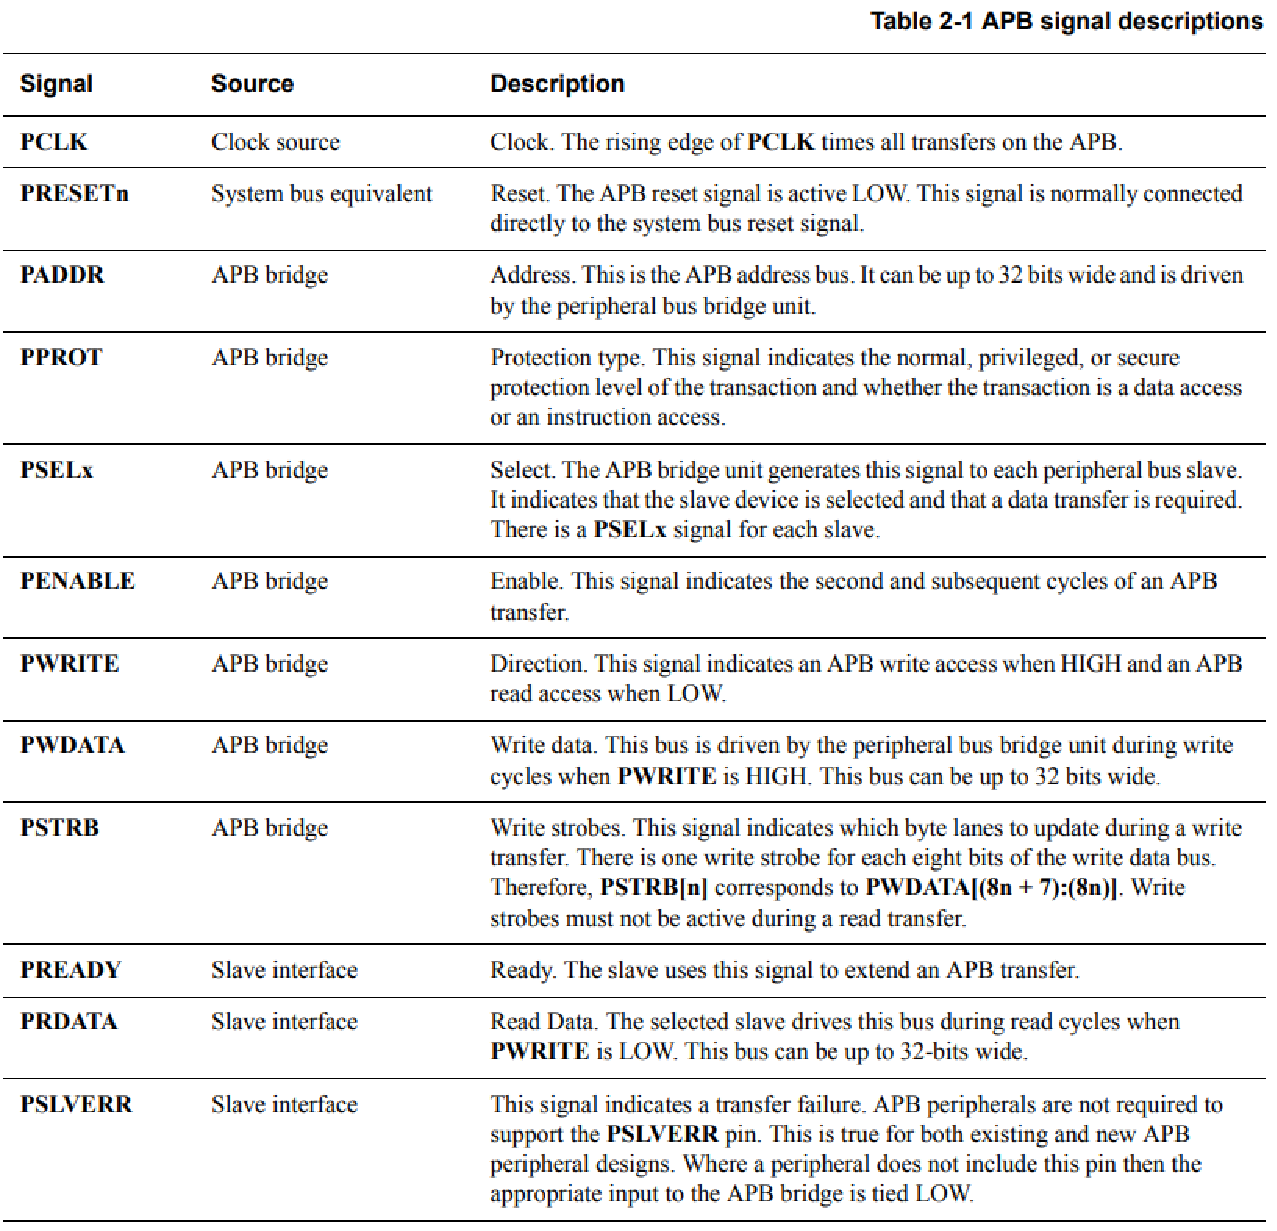
\includegraphics[width=\linewidth]{subfiles/imgs/IP_Blocks_Pics/apb_signals.pdf}
    \caption{Table of signals in the APB protocol (Courtesy of ARM \cite{apbReference}).}
    \label{fig:apb_signals}
\end{figure}

The protocol contains two individual buses for read and write operations. However, only one of these transfers can be executed at a time. The read and write transfer using the APB protocol with no wait cycles can be seen in figure \ref{apb_transfers_no_wait}.

\begin{figure}[H]
     \centering
     \begin{subfigure}[b]{0.49\textwidth}
         \centering
         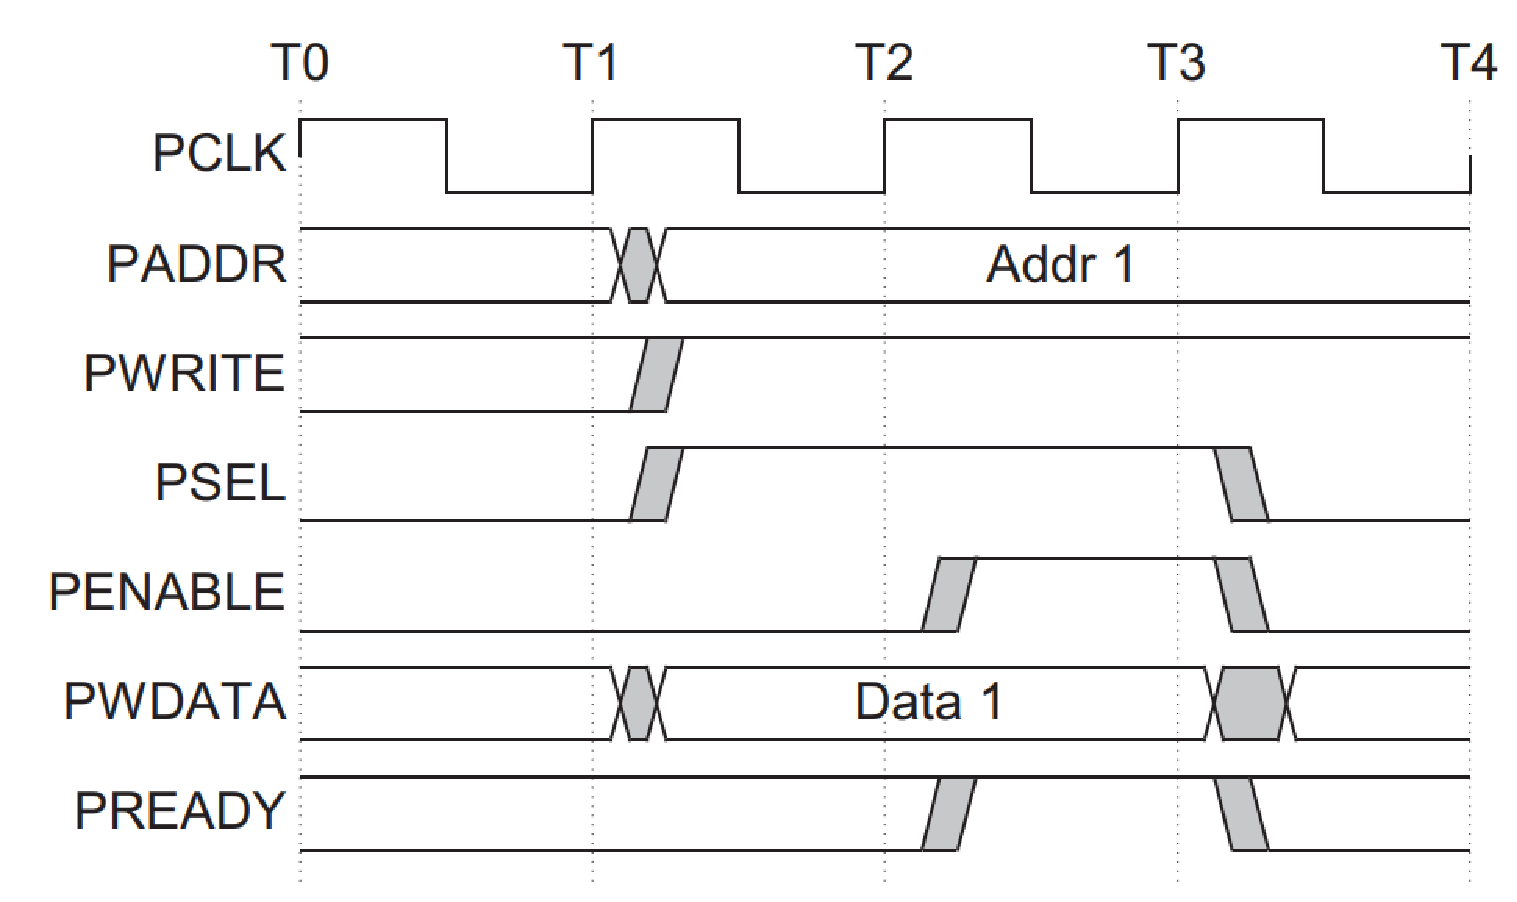
\includegraphics[width=\textwidth]{subfiles/imgs/IP_Blocks_Pics/apb_write_no_wait.pdf}
         \caption{Write transfer}
         \label{fig:apb_write_no_wait}
     \end{subfigure}
     \hfill
     \begin{subfigure}[b]{0.49\textwidth}
         \centering
         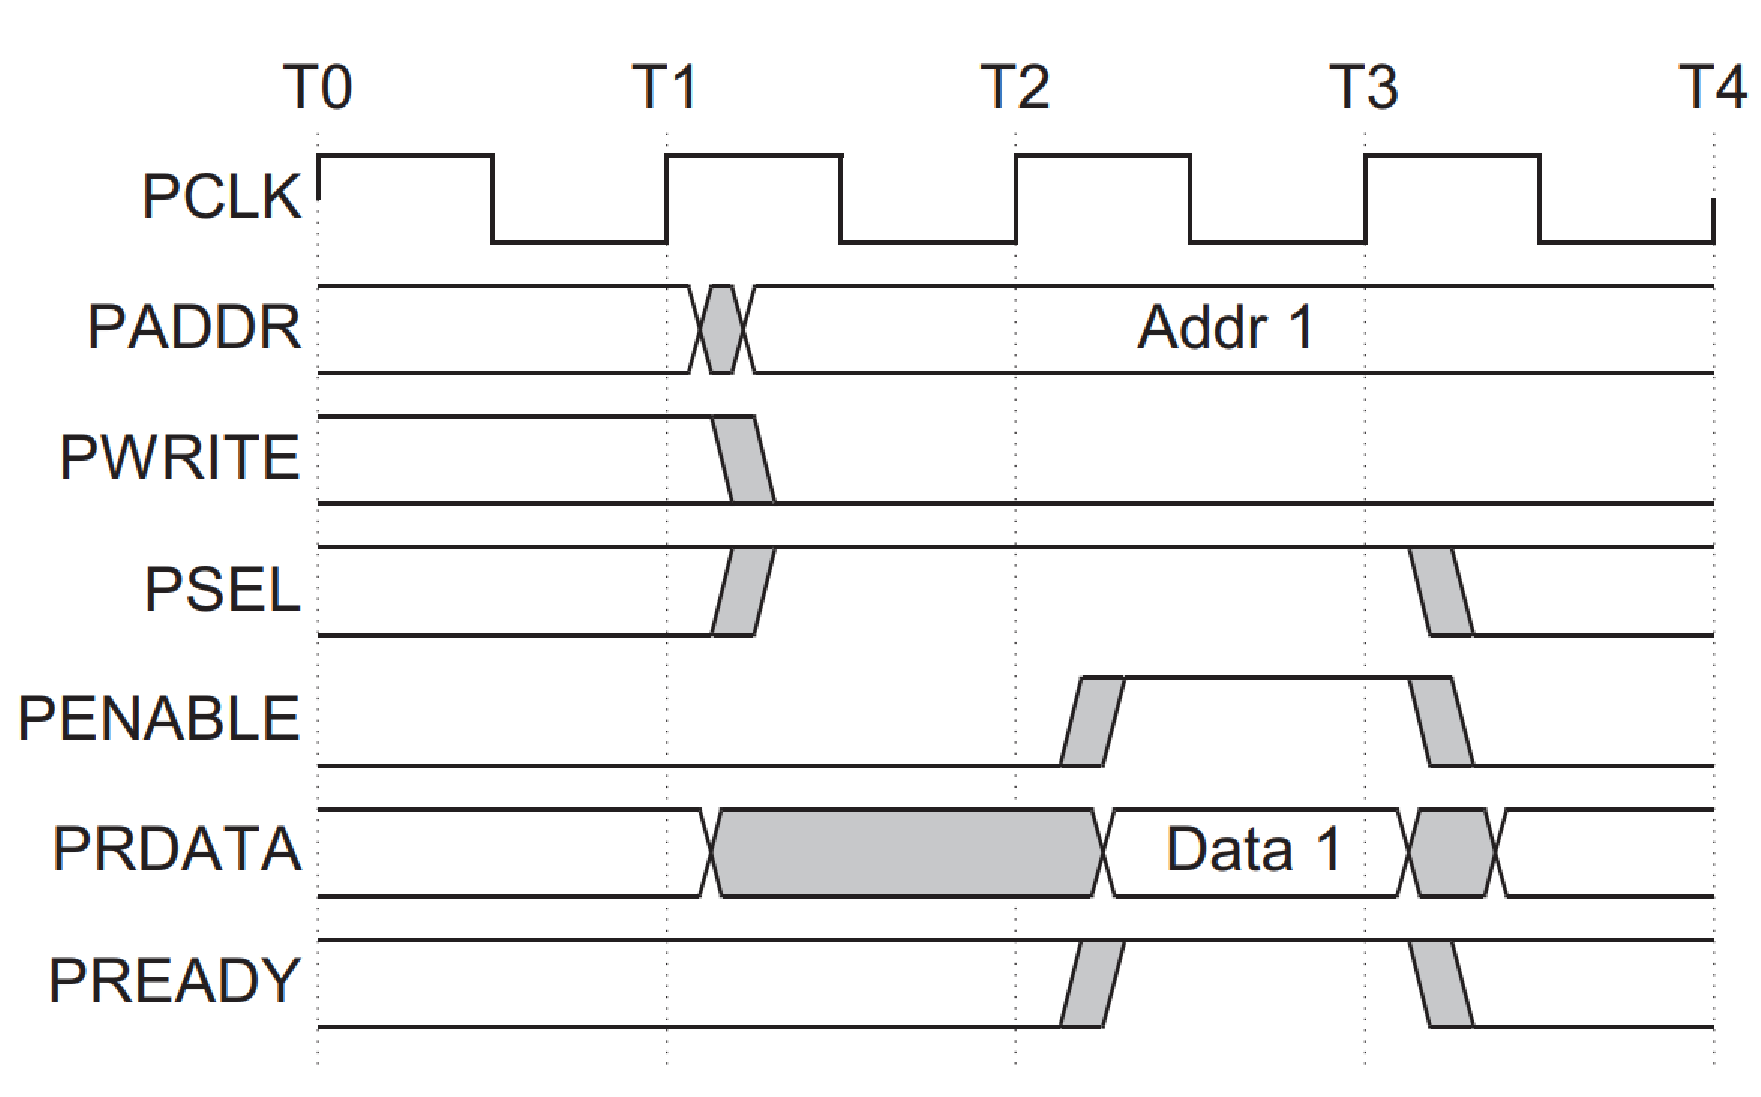
\includegraphics[width=\textwidth]{subfiles/imgs/IP_Blocks_Pics/apb_read_no_wait.pdf}
         \caption{Read transfer}
         \label{fig:apb_read_no_wait}
     \end{subfigure}
     \hfill
     \caption{Shows the basic transfers of the APB protocol with no wait cycles (Courtesy of ARM \cite{apbReference}).}
     \label{apb_transfers_no_wait}
\end{figure}

Wait cycles can be introduced if the slave does not assert the PREADY signal. However, the way the APB protocol is connected to the CPU will cause stalling of the entire CPU until the PREADY is asserted and the transfer is completed. A timeout could partially solve this by limiting the stalling period, but this does not fix the problem but only reduces it. Therefore it is chosen that the IP block as a general rule should always have PREADY asserted, as to ensure no stalling of the system. Instead in the case of a bad transfer due to no data available or similar situations, the PSLVERR signal is utilized and the IP block will then assert this signal to indicate that the transfer has failed. This introduces problems as this signal does not indicate why the transfer failed. However, it does remove the stalling. Therefore, this method is chosen. 

The APB bus will not be triplicated as this will connect all peripherals to the core and the length can therefore be quite significant, which will result in a larger area used and more complex routing. Instead, an encoding approach is used. Every byte of the bus is encoded using Hamming codes, which are capable of single error correction and double error detection. This approach uses the same logic developed later for radiation-tolerant memories. 

